\documentclass[11pt,fleqn]{article}
% \documentclass[smallextended]{svjour3}

\textheight=23.3cm 
\textwidth=16.5cm 
\topmargin=-15mm 
\oddsidemargin=0cm 

\usepackage{enumerate}
\usepackage{amsmath}
\usepackage{amssymb}
\usepackage[utf8x]{inputenc}
\usepackage[dvipsnames]{xcolor}
\usepackage{bbm}
\usepackage{ulem}
\usepackage{graphicx}
%This package is dated and it is giving me problems
%\usepackage{subfig}
\usepackage{wrapfig}
\usepackage{pdflscape}
\usepackage[sidewaysfigure]{rotating}
\usepackage{natbib}
%\usepackage{amsthm}
%\usepackage{setspace}
\usepackage{multirow}
\usepackage{subcaption}
\newcommand{\tb}{\hspace*{3mm}}
\bibpunct{(}{)}{;}{a}{,}{,}
\parskip=3mm 
\parindent=5mm 
\baselineskip=17pt

\usepackage{amsthm}
\newtheorem{assumption}{Assumption}
\newtheorem{definition}{Definition}
\newtheorem{proposition}{Proposition}
\newtheorem{corollary}{Corollary}
\newtheorem{lemma}{Lemma}
\newtheorem{theorem}{Theorem}
\renewcommand{\qedsymbol}{\textit{Q.E.D.}}

\DeclareMathOperator*{\argmax}{arg\,max}
\DeclareMathOperator*{\argmin}{arg\,min}

\usepackage{algpseudocode}
\usepackage{algorithm}

\usepackage{hyperref}
\hypersetup{
  pdftitle={Divide and Conquer},    % title
  pdfauthor={Robert Kirkby},     % author
  %hyperfootnotes=false,
  %hyperindex=true,
  %hyperfigures=true,  
  colorlinks=true,                % makes links a coloured word, rather than putting coloured boxes around them
  linkcolor=black,                % makes internal links black
  citecolor=black,                % makes citations black
  urlcolor=blue,                 % color of external links
  breaklinks=true                 % allow links to be brocken across multiple lines      
}


\begin{document}


%===============================
\newcommand{\rob}[1]{{\noindent\color{blue}\bf #1}}
\newcommand{\robc}[1]{{\noindent\color{blue}\bf R: #1}}
%===============================

\title{Grid Interpolation Layer}
\author{Robert Kirkby\thanks{Thanks to AAA. Thanks to R\={a}poi at Victoria University of Wellington for the use of their computing facilities. Kirkby: Victoria University of Wellington. Please address all correspondence about this article to Robert Kirkby at $<$robertdkirkby@gmail.com$>$,
\href{http://www.robertdkirkby.com}{robertdkirkby.com}.} }
\date{\today}
\maketitle

\begin{abstract}
Interpolation is a powerful technique for improving the accuracy-runtime (and accuracy-memory) trade-off when solving value function iteration problems. But standard interpolation routines are highly serial and thus not appropriate for the gpu. This brief pdf describes the 'grid interpolation layer' for the GPU that is implemented in VFI Toolkit.
\end{abstract}

\noindent {\bf Keywords:} Value Function Iteration, Grid Interpolation Layer, VFI Toolkit.

% \noindent {\bf JEL Classification:} E00; C63; C15; E24.

\thispagestyle{empty}

% %==============================================================================
% \newpage
% {
% \small
% \parskip=0cm
% \parindent=0cm
% \tableofcontents
% }
% %==============================================================================


\newpage
\baselineskip=17pt
% \setcounter{page}{1}

% \section*{Introduction}
This document is going to largely assume you are already familiar with the concept of interpolation. The basic idea when used in value function iteration is that we have a grid on assets (the endogenous state) and we know the next period expected value function on that same grid for next period assets. If we just restrict our choice of next period assets to fall on the grid, we get the pure discretization that is the basic algorithm of VFI Toolkit. To make the solution more accurate (without changing the grid we are using) we would like to choose values of next period assets without restricting them to be on the grid. This requires evaluating two things at potential values of next period assets (so we can find the optimal value for next period assets), the return function and the expected next period value function. Evaluating the return function off the grid is trivial, it is a known function and so we can just evaluate this function. Evaluating the next period expected value function is trickier, we only know the value function at the points corresponding to the grid on next period assets, so for values not on this grid we must perform interpolation.

So we will use interpolation to evaluate the expected next period value function in terms of next period assets at points between the grid on next period assets. The question then is how to pick which values for next period assets to try, so as to find the optimal value for next period assets (given a value for todays assets). Standard CPU implementations involve an initial guess for next period assets, call it $x^0$, and then update this guess repeatedly as $x^1$, $x^2$, $x^3$, until convering to an optimal $x*$; this might be done using bisection search, golden search, Newton-Raphson, or many other optimization algorithms. This would be a bad idea on the GPU, as $x^0$, $x^1$,$\dots$, $x^m$ are highly serial (we have to finish calculating $x^m$ before we can calculate $x^{m+1}$) with any of these approaches.

Before proceeding to introduce an approach to interpolation that is highly parallel and hence GPU friendly, let's do a bit of notation to set things up. Let our grid on assets be $\{a_1,a_2,\dots,a_n\}$, and use $i=1,\dots,n$ as to index these grid points. We will use this same grid on next period assets, but refer to it as $\{aprime_1,aprime_2,\dots,aprime_n\}$.\footnote{In theory we could have these being two distinct grids, and they could have different numbers of grid points. Here we assume they are the same grid as it simplifies the exposition, and as that is what the code does.} The grid is assumed to be stictly increasing, so $a_i<a_{i+1}$ for all $i=1,\dots,n-1$.

For interpolation to work on the GPU, we need to use a more parallel/less serial approach. The idea implemented as 'grid interpolation layer' in VFI Toolkit is that we first solve the standard pure discretization problem as the 'first layer'; we already know $E[V(aprime_i)]$ for all the points on the next period assets grid. For a given value of todays assets, this will give us an optimal on-the-grid point for next period assets, call it $aprime_i$. We will then perform a 'second layer' by creating a finer grid around $aprime_i$; based on an assumption of monotonicity we know from the fact that $aprime_i$ was on-the-grid-optimal that the true optimal value will lie in the range ($aprime_{i-1},aprime_{i+1}$). So our second layer will consider the points $aprime_{i-1}$, $a_{i-1,1}$, $a_{i-1,2}$,$\dots$,$a_{i-1,n2}$, $aprime_i$, $a_{i,1}$, $a_{i,2}$,$\dots$,$a_{i,n2}$, $aprime_{i+1}$; note that this is the points $aprime_{i-1}$ and $aprime_i$ with $n2$ points between them, and then the points $aprime_i$ (not duplicated) and $aprime_{i+1}$ with $n2$ points between them, for a total of $2*n2+3$ points in the 'second layer' grid on next period assets. We can simply evaluate the return function at each of these points (by function evaluation) and use linear interpolation to evaluate the expected next period value function at each of these points, we can then find the optimal next period assets from among these 'second layer' grid points. To keep things simple, we will assume that the $n2$ second layer points are always evenly spaced beween the first layer grid points.\footnote{This is obviously not important to being able to do grid interpolation layer, just keeps things simple in the code.}

So to implement this, we solve the 'first layer' considering only values of $aprime$ on the grid. Then in the second layer we consider only values of $aprime$ that are on the second layer grid, which puts $n2$ points between the first layer grid points above and below the first layer grid point that was found to be optimal in the first layer. Note that the effect of all of this is that we are implicitly considering the 'fine' grid on aprime that is given by the Matlab code $aprime\_{}grid=interp1(1:1:n,a\_{}grid,linspace(1,n,n+n2*(n-1)))$, which contains $n2*(n-1)+n$ points (the $n$ points on the first layer grid, plus $n2$ points between each of them). But by doing it in two layers we only actually end up considering $n+(3+2*n2)$ points, and so runtimes are fine. As an example, we might use 301 points in the first layer and 20 in the second, meaning we are implicitly considering a grid of 6301 points on next period assets, but only have to actually evaluate 344 points in two layers. Most important for the GPU, there are just two steps in serial, and everything else is done in parallel within these two layers.

\newpage

\subsection*{Intuition}
Imagine we are at a particular point in today's state-space, and we are deciding which value (or index) of $aprime$ to choose. Say the first layer grid on $aprime$ has seven points, represented in Figure \ref{fig:firstlayer} as seven numbered circles. Each circle has an associated value of the return function $F$ and of the next period expected value function $EV$. Say it turns out that the third circle is the optimal choice on the first layer grid (the first layer of the grid interpolation layer algorithm). We are then in the situation of Figure \ref{fig:secondlayer}: we keep the third circle together with the first layer circles immediately above and below it, and between each consecutive pair we insert five smaller circles, which form the second layer (the grid interpolation layer itself). In Figure \ref{fig:secondlayer} the second layer optimum is at $2.4$, where the integer part is the lower first layer grid point and the decimal counts the small circles between it and the next first layer grid point upwards, so the chosen point is two small circles below the third coarse circle that was optimal in the first stage.

\begin{figure}[h]
\caption{Grid Interpolation Layer - Intuition}
\centering
\begin{subfigure}[c]{0.45\textwidth}
\centering
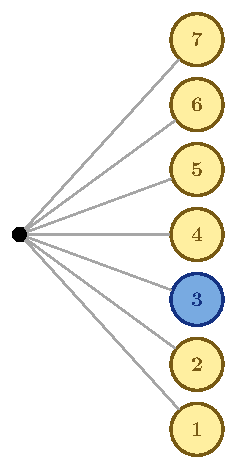
\includegraphics{Graphs/FigureX.pdf}
\caption{First layer: the seven points of the coarse grid on $aprime$. The third circle (blue) is the first layer optimum.}
\label{fig:firstlayer}
\end{subfigure}
\hfill
\begin{subfigure}[c]{0.45\textwidth}
\centering
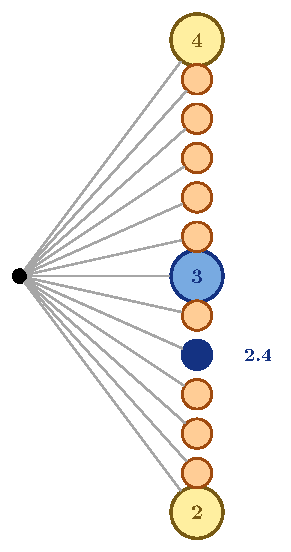
\includegraphics{Graphs/FigureY.pdf}
\caption{Second layer: the first layer optimum (circle $3$, blue) and its two neighbours, with five second layer points (orange) between each consecutive pair of first layer points. The second layer optimum at $2.4$ is shown in dark blue.}
\label{fig:secondlayer}
\end{subfigure}
\end{figure}

\newpage

\subsection{Pseudocode}
This is the pseudocode for solving a simple finite horizon value function problem. One endogenous state, no decision variable, one markov shock. Let $a\_{}grid=\{a_1,\dots,a_n\}$ be the grid on assets (for both today and tomorrow), and  $z\_{}grid=\{z_1,\dots,z_m\}$ be the grid on the markov shock and let $pi\_{}z$ be the associated markov transition matrix.

Let $\Theta$ be all the parameters of the model, and let $\theta_j$ be the values of those parameters which are relevant in period $j$.\footnote{So if a parameter is independent of age, then it is just in $\theta_j$ as is. If a parameter depends on age, then only the value relevant to age $j$ is in $\theta_j$.}
\begin{algorithmic}
\State{Create the fine grid: $afine\_{}grid=interp1(1:1:n, a\_{}grid, linspace(1,n, n+(n-1)*n2))$.}
\For{$j$ count backward from $N_j$ to $1$}
   \State Get $\theta_j$ from $\Theta$
   \For{All values $z$}
    \State Calculate $EV_j(a',z)=E[V_{j+1}(a',z')]$ \Comment For $j=N_j$ this is zero
    \State Interpolate $EV_j(a,z)$, which exists on the first layer grid,
    \State $\quad$ $\quad$ onto the entire fine grid to get $\hat{EV}_j(a,z)$.
     \For{All values of $(a,z)$}
     \State \textbf{First Layer}
     \State Solve for optimal $aprime$ on grid:
     \State $\quad$ $\quad$ $g^1_{j}(a,z)=argmax_{i=1,...,n} F(a\_{}grid(i),a,z) + \beta EV_j(a\_{}grid(i),z)$
     \State Note: $a\_{}grid(i)$ is $i-th$ grid point in grid on $aprime$, and we
     \State $\quad$ $\quad$ get $g^1_{j}(a,z)$ as an index for the optimal aprime, not a value.
     \State \textbf{Second Layer}
     \State Create second layer grid:
     \State $\quad$ $\quad$ $aL2\_{}ind=(g_j(a,z)-2)*(n2+1)+(1:1:(3+2*n2))$  \Comment fine-grid indices for the second-layer band; given $(a,z)$
     \State $\quad$ $\quad$ $aL2\_{}grid=linspace(g_j(a,z)-1,g_j(a,z)+1,3+2*n2)$  \Comment Not used, illustrates what $aL2\_{}ind$ corresponds to when it indexes the fine grid.
     \State Solve for optimal $aprime$ on second layer grid:
     \State $\quad$ $\quad$ $g^2_{j}(a,z)=argmax_{i=1,...,3+2*n2} F(afine\_{}grid(aL2\_{}ind(i)),a,z) + \beta \hat{EV}_j(aL2\_{}ind(i),z)$
    \EndFor
   \EndFor
  \EndFor
  \State Turn the two layer optimal indexes $[g^1_1,g^1_2,...,g^1_{N_j}]$ and  $[g^2_1,g^2_2,...,g^2_{N_j}]$ into some optimal policy $[g_1,g_2,...,g_{N_j}]$. \Comment Following three lines explain this.
  \State Convert $(g^1_j(a,z), g^2_j(a,z))$ into $(lower\_{}index, second\_{}layer\_{}index)$:
  \State $\quad$ $\quad$ if $g^2_j(a,z) \leq n2+1$: $lower\_{}index=g^1_j(a,z)-1$, $second\_{}layer\_{}index=g^2_j(a,z)$
  \State $\quad$ $\quad$ else: $lower\_{}index=g^1_j(a,z)$, $second\_{}layer\_{}index=g^2_j(a,z)-(n2+1)$
  \\ \Return $[V_1,V_2,...,V_{N_j}]$, $[g_1,g_2,...,g_{N_j}]$ \Comment $V$ are the max from second stage ($g$ was argmax)
\end{algorithmic}
The notation $EV_j(a',z)=E[V_{j+1}(a',z')]$ is capturing that since $z$ is a markov, the expected value $E[V_{j+1}(a',z')]$ can be expressed as a function of $(a'z)$ (by taking expectations over $z'$ using the transition matrix $pi\_{}z$ which depends on $z$); this follows from $z$ is markov.

One thing worth discussing is what form the optimal policy $[g_1,g_2,...,g_{N_j}]$ should be stored in. I choose to store it as the 'index of the lower grid point of $a\_{}grid$' (which is a number from 1 to $n-1$) together with the index of the second layer (which is a number from 1 to $n2+2$). When using the policy to create the agent distribution we will want the 'upper and lower grid points of $a\_{}grid$' (the upper is just lower plus 1, so that is easy) and the 'weights' which can be trivially calculated from the second layer index (weight of lower grid point is $1-(second layer index-1)/(n2+1)$; because we placed the second layer points evenly spaced). When using the policy to evaluate fns on the agent dist we want the aprime value, which we can trivially do by creating the 'fine' grid, $aprime\_{}grid=interp1(1:1:n,a\_{}grid,linspace(1,n,n+n2*(n-1)))$ and getting the index for the fine grid as 'fine grid index'=$(n2+1)*($'index of the lower grid point of $a\_{}grid$'$ -1)+$'second layer index', then simply use the index for the fine grid to get the grid value from the fine grid. Since we created the indexes while solving the value fn problem,\footnote{When we solve the first layer we got the 'midpoint', switching this to the 'lower grid point' just requires substracting one from it.} it makes sense to store these, and only get the weights as needed for the agent dist.

One minor detail I have omitted above. The index we get solving the first layer is a 'midpoint' for the second layer. But if it is at the edges of the grid we cannot use it as a midpoint for the second layer. So just check if it is the first/last grid point, and if so then add/subtract one, respectively, before using it as midpoint for second layer.

\subsection*{Decision Variables and Exogenous Shocks}
The obvious approach is to apply this idea 'conditional on' any decision variables and exogenous shocks. This is exactly how VFI Toolkit handles it.

Note that when there is a decision variable this does rather change how the 'first layer' is done, relative to pure discretization. In pure discretization we would find the optimal $(d*,aprime*)$, which is a single value for each of $d$ and $aprime$ (for each point in todays state-space). But now in the first layer we have to find the optimal $aprime$ for each possible $d$, so $aprime*(d)$, which is a single value of $aprime$ for each possible value of $d$, and the in the second layer we create a different second layer grid for each possible value of $d$. The second layer is more standard as now we just want the optimal $(d*,aprime*)$.

\subsection*{Linear interpolation and evenly spaced points}
Until now we have not specified how the interpolation should be done. In VFI Toolkit linear interpolation is used.

Everything described above could easily be done without the second layer grids being evenly spaced, and by using any interpolation other than linear. The evenly spaced grids are intuitive and easy, and it is not obvious that there is an alternative choice that would meaningully improve performance (the choice of a good $a\_{}grid$ is likely much more important, as are the choice of $n$ and $n2$). As for linear interpolation, you could easily use something else. I have not tested the alternatives: they will increase runtime and improve accuracy, but will the improved accuracy be worth the increased runtime? The code in VFI Toolkit does the interpolation using Matlab's 'interp1()', so if anyone does want to test them it is as trivial as changing \textit{interp1(a\_{}grid,EV,aprime\_{}grid)} to \textit{interp1(a\_{}grid,EV,aprime\_{}grid,'spline')}, or similar (note, not all the interpolation methods in \textit{interp1()} work with GPU).

\subsection*{VFI Toolkit}
You turn on the use of grid interpolation layer by setting $vfoptions.gridinterplayer=1$, and you must also say what the number of points to use in the second layer between the first layer grid points, $n2$ above, which you do by setting, e.g., $vfoptions.ngridinterp=20$.

Normally the first dimension of 'Policy' (the policy function created by the value fn iteration commands) contains the indexes for each of the policies (so if you have one decision variable and one endogenous state, there would be two policies and the second would correspond to endogenous state). When you use the grid interpolation layer the endogenous state is now two indices, one for the 'lower grid point of first layer' and the second for the 'second layer index'; these are described above.

Note that because the interpretation of Policy has changed, we need to tell all the other commands about it so they know what to do. Hence you also need to set $simoptions.gridinterplayer=vfoptions.gridinterplayer$ and $simoptions.ngridinterp=vfoptions.ngridinterp$.

\subsection*{Combination with divide-and-conquer}
Notice that the first layer is essentially just the pure discretization problem. So we can apply divide-and-conquer to the first layer just as we would to any other problem. This gives us an algorithm where we do two-layer grid interpolation and use divide-and-conquer on the first layer; the second layer just standard. This is what VFI Toolkit does if you set both $vfoptions.divideandconquer=1$ and $vfoptions.gridinterplayer=1$.

\subsection*{Agent Dist and EvalFnOnAgentDist}
When using the grid interpolation layer ($vfoptions.gridinterplayer=1$) the $Policy$ is now the 'lower grid point index' and the 'interpolation layer index' for the next period endogenous state. We can simply keep the 'lower grid point index' and convert the 'interpolation layer index' into a probability of the lower grid point. We then use the 'n probs' setting for iterating on the agent distribution. This is explained in the \href{https://github.com/vfitoolkit/Pseudocodes/blob/main/VFI_PseudoCodes.pdf}{Psuedocodes pdf} for VFI Toolkit.


For evaluating functions on the agent distribution we just need to convert $Policy$ to $PolicyVals$ (from indexes to values) and then the rest of the commands are standard. When using the policy to evaluate fns on the agent dist we want the aprime value, which we can trivially do by creating the 'fine' grid, $aprime\_{}grid=interp1(1:1:n,a\_{}grid,linspace(1,n,n+n2*(n-1)))$ and getting the index for the fine grid as 'fine grid index'=$(n2+1)*($'index of the lower grid point of $a\_{}grid$'$ -1)+$'second layer index', then simply use the index for the fine grid to get the grid value from the fine grid


\subsection*{How to deal with -Inf?}
To get the basic idea of what can go wrong when we have $-\infty$, imagine the following. We have a model in which 'assets' is an endogenous state. The coarse (first layer) grid has eleven points, $a\_{}grid=[0,10,20,\dots,90,100]$. Say the model has a constraint that you are not allowed to choose assets above $97$, so the return function gives $-\infty$ whenever $aprime>97$. The problem is that, say, you choose $aprime=97$; then when we interpolate this back onto $a\_{}grid$ during simulation/iteration of the agent distribution, some mass ends up at $a=100$. Despite the fact that no agent is allowed to choose $aprime>97$, and no agent does, some agents still end up with $a=100$. This is what we want to eliminate by being careful in how the grid interpolation layer handles $-\infty$.

To understand how to handle $-\infty$ we need to consider two possibilities: that the $-\infty$ comes from the next period value function, or that the $-\infty$ comes from the return function. To be able to consider these, we revisit Figure \ref{fig:secondlayer}. In Figure \ref{fig:splitcells} we have replaced each circle by a pair of circles joined by a $+$ sign: the left circle holds the return function value ($R_2, R_{2.1},\dots$) and the right circle holds the next period (expected) value function value ($V_2, V_{2.1},\dots$). The optimal choice is the row that gives the largest $R+\beta V$. The key difference between the two cases is that we only know $V$ on the coarse grid and have to interpolate $V$ at the second layer points, whereas $R$ can be calculated exactly at the second layer points (because we know the return function).

\begin{figure}[h]
\centering
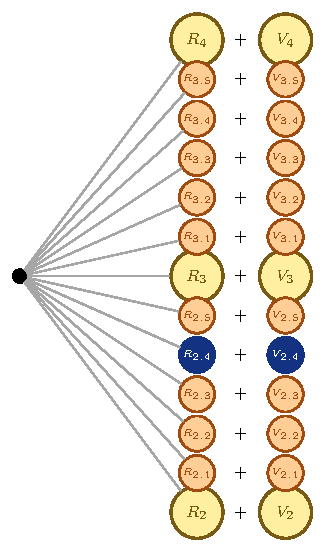
\includegraphics{Graphs/FigureZ.pdf}
\caption{Paired-circle view of Figure \ref{fig:secondlayer}: each row gives a candidate $aprime$ as a pair of circles, the left holding the return function value $R$ and the right holding the next period value function value $V$. The optimal choice is the row maximising $R+\beta V$.}
\label{fig:splitcells}
\end{figure}

First, in Figure \ref{fig:vinf} consider the case in which $-\infty$ appears in the next period value function, say the upper $V_4$ (coloured black to show it is ruled out by being $-\infty$). Because $V_4$ is $-\infty$, we cannot meaningfully interpolate to obtain values for $V_{3.1},\dots,V_{3.5}$, and so we conservatively assume that they are all $-\infty$ as well (hence they are now all black). Other than filling in $-\infty$ for $V_{3.1},\dots,V_{3.5}$, this does not require any change to the algorithms we have seen so far.

\begin{figure}[h]
\centering
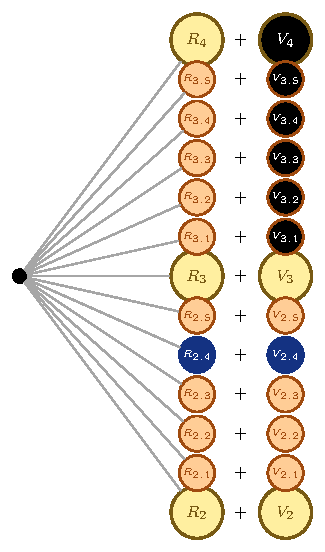
\includegraphics{Graphs/FigureU.pdf}
\caption{The case where the next period value function takes the value $-\infty$ at $V_4$. The values $V_{3.1},\dots,V_{3.5}$ would have to be obtained by interpolating between $V_3$ and $V_4$; since $V_4=-\infty$ we conservatively set them all to $-\infty$.}
\label{fig:vinf}
\end{figure}

Second, in Figure \ref{fig:rinf} consider the case in which $-\infty$ appears in the return function, say the lower $R_2$ (coloured black to show it is ruled out by being $-\infty$). Unlike the previous case, we can still calculate all of $R_{2.1},\dots,R_{2.5}$, because these simply involve evaluating the (known) return function. This is the 'tricky' situation, in the sense that we have to decide what to do here, unlike the previous case where the conservative answer was essentially forced on us. We have come up with four possibilities.

\begin{figure}[h]
\centering
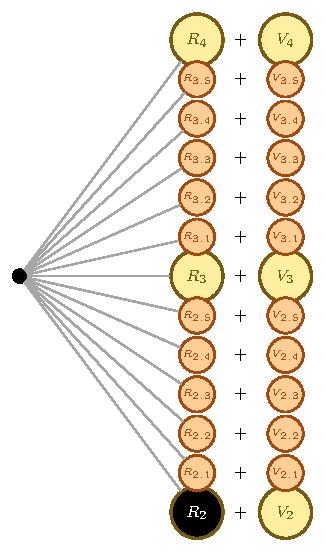
\includegraphics{Graphs/FigureT.pdf}
\caption{The case where the return function takes the value $-\infty$ at $R_2$. Unlike the value function case, the intermediate return function values $R_{2.1},\dots,R_{2.5}$ can still be evaluated exactly. But the question is what do do here?}
\label{fig:rinf}
\end{figure}

The first possibility is simply to do the same as we did when the next period value function was $-\infty$, namely to deliberately contaminate all the intermediates ($R_{2.1},\dots,R_{2.5}$) with $-\infty$. This is very simple to implement, but it 'gives up' a lot of information, since we are not taking advantage of what we know about the return function.

The second possibility (which is what the original implementation in VFI Toolkit did) is simply to pick the best interpolation point and then proceed as usual: we know all the intermediate $R$ values by evaluation and all the intermediate $V$ values by linear interpolation. This gives the most accurate value function. The drawback only becomes apparent when we combine this with simulating/iterating the model forward: the agent is placed on the two neighbouring coarse grid points with some mass on each, which is effectively saying that with positive probability the agent has chosen a policy that gives a return of $-\infty$ in order to be able to reach the neighbouring coarse grid point. This is precisely the problem of the 'limit of 97 dollars, but some end up on 100' that we saw at the beginning of this section. So while this option gives the most accurate value function, it comes at the cost of 'leaking' a small fraction of agents into 'impossible' behaviour.

A third possibility is to still use the 'evaluate the return function on all intermediates and pick the optimum' approach of the second possibility, but to add a 'flag' that records the fact that one of the two neighbouring coarse grid points is 'impossible'. We then keep the maximum accuracy of the value function, but when iterating the agent distribution we use the flag to put zero mass on the 'impossible' coarse grid point and full mass on the other (so the flag overrules the standard linear interpolation back onto the coarse grid whenever one of the neighbouring coarse grid points represents an 'impossible' policy). This is excellent from an accuracy perspective: we get the best value function and we avoid leaking into impossible grid points. The weakness is a subtle inconsistency between the agent's expectations and what actually happens to them: when an intermediate grid point is chosen the agent's expectations put probability on both neighbouring coarse grid points, but the simulation sends the agent entirely to one of the two coarse neighbours, avoiding the impossible one.

This leads to a fourth possibility. We let agents choose intermediate grid points, but in the cases where a $-\infty$ in the return function rules out a neighbouring coarse grid point, we construct the interpolated value function values using the same 'all mass on the remaining neighbour, zero on the impossible one' weights that we will use when iterating the agent distribution. This seemed clever at first, but in practice it collapses into the first possibility roughly half of the time. The return function is monotone decreasing in next period endogenous state in (effectively all) economic models, so if we make the next period value function a constant across the interpolation points (which is what putting weights of one and zero on the two neighbours achieves), then if the $-\infty$ is on the upper coarse neighbour we will simply pick the lower coarse neighbour as the optimum. If the $-\infty$ is on the lower coarse neighbour, the behaviour is slightly different: we choose the first interpolation point above the impossible coarse neighbour (or, more precisely, the lowest interpolation point whose return function value is not $-\infty$).

So what to do? We have four options and no clear winner. Possibilities two and three give the most accurate value function, but possibility two 'leaks' into 'impossible' states during simulation/iteration of the agent distribution, so we consider it ruled out. Possibility three carries a small 'expectations' distortion, in that the value function and what actually happens to the agent differ subtly in terms of the probabilities placed on the 'impossible' coarse neighbour. Possibility four is, to our mind, better than possibility one: it is slightly more complicated to code but not in a way that would ever show up in runtime, and it provides marginally more accuracy. So we are down to a choice between three and four.

Fundamentaly, what we are seeing here is that there is no easy way to deal with interpolation when you have a finite number on one side and a $-\infty$ on the other. Evaluating the return fn exactly at the intermediate points at first glance allows us to side-step this, but looking closely we see that actually this just shifts the problem into the simulation/interpolation where we linearly interpolate back onto the grid.


\subsubsection*{Explanation of how this gets coded}
There are two distinct sources of $-\infty$ that need to be handled when using the grid interpolation layer: the next period value function $EV_j(aprime,z)$ may take a value of $-\infty$ at one of the first layer grid points (for example because that state is unreachable or absorbing into an infeasible region), and the return function $F(aprime,a,z)$ may take a value of $-\infty$ at one of the first layer grid points (typically because $aprime$ violates a constraint at the current $(a,z)$, such as a borrowing constraint or a non-negativity constraint on consumption).

These two cases are handled differently in the second layer. When $EV_j$ is $-\infty$ at a first layer grid point we must do something explicit, because the second layer uses linear interpolation of $EV_j$. The choice made is conservative: whenever one of the two first layer grid points either side of a second layer interval is $-\infty$, we treat the entire interval between them as $-\infty$ rather than interpolating against the $-\infty$ value (which would otherwise propagate $-\infty$ to every second layer point in the interval and prevent us from distinguishing between them). When $F$ is $-\infty$ at a first layer grid point we do not need any special handling, because the return function is evaluated exactly at every second layer point (rather than interpolated) and so a $-\infty$ at a first layer point places no restriction on the second layer points. We simply let the maximisation discard them. The resulting Policy is as accurate as possible, while remaining conservative with respect to states which should genuinely be $-\infty$.

These two choices are each individually fine. However, they interact badly with the way the agent distribution is iterated. The standard treatment of the agent distribution under the grid interpolation layer is to keep the lower first layer grid point and convert the second layer index into a probability weight on the lower and upper first layer grid points (the 'n probs' setting described above). The problem is the following: suppose at some $(a,z)$ the optimal $aprime$ lies on a second layer point in the interval $(aprime_i,aprime_{i+1})$, and that $F(aprime_{i+1},a,z)=-\infty$ but $F$ is finite at the chosen second layer point and at $aprime_i$. The Policy is correct, in the sense that the chosen second layer point itself is feasible. But when iterating the agent distribution we then place a non-zero weight on the first layer grid point $aprime_{i+1}$, which is exactly the point at which $F=-\infty$. We are effectively saying that with positive probability the agent chose an $aprime$ at which the return function is $-\infty$. This causes agents to leak into states which are infeasible at the current $(a,z)$.

One possible fix would be to rule out any second layer optimum whenever a neighbouring first layer grid point has $F=-\infty$, forcing the Policy back onto a first layer grid point in such cases. This eliminates the leakage, but at a substantial cost to the accuracy of the Policy: we lose the second layer entirely whenever we are close to a constraint, which is exactly the region where it matters most. Instead, we keep the second layer index in the Policy (so plots of Policy and statistics computed using $FnsToEvaluate$ retain the full accuracy of the grid interpolation layer), but we modify how the second layer index is translated into weights when iterating the agent distribution. Specifically, in the case where the upper first layer grid point has $F=-\infty$ we move the entire probability mass to the lower first layer grid point, and symmetrically for the lower first layer grid point.

To implement this, when the grid interpolation layer is being used $Policy$ now carries an additional row containing a flag with three possible values. A flag value of $2$ indicates the usual case: convert the second layer index into weights on the lower and upper first layer grid points in the standard way. A flag value of $1$ indicates that all weight should be placed on the lower first layer grid point. A flag value of $3$ indicates that all weight should be placed on the upper first layer grid point. The flag is set during the value function iteration based on the values of $F$ at the neighbouring first layer grid points, and is then used whenever the policy is converted into transition weights on the first layer grid (so during agent distribution iteration, but not when evaluating functions on the agent distribution, where the fine grid value of $aprime$ is used directly).

It is useful to think about this in terms of how the algorithm handles a constraint that tips from non-binding to binding between two first layer grid points. There is necessarily some 'fuzziness' on one side or the other of the true tipping point, because the agent distribution lives on the first layer grid. The original approach was to allow fuzziness by breaching the constraint as far as the next first layer grid point (placing some weight on the infeasible upper grid point). Simply ruling out the second layer optimum, as in the first alternative above, would amount to enforcing the constraint as far as the previous first layer grid point at \textit{both} the Policy and the agent distribution stages. The approach actually taken places no fuzziness in the Policy itself, and enforces the constraint as far as the previous first layer grid point only when iterating the agent distribution. As the first layer grid is refined all three approaches converge; the question is which behaves best when the first layer grid is genuinely coarse, and the chosen approach strikes a better balance in that regime.

This change is largely invisible at the user level. The two exceptions are: any model in which the leakage was occurring will now give corrected results (so results may differ from those produced by earlier versions of the toolkit, and the new results are the correct ones); and any $Policy$ saved from an earlier version of the toolkit will no longer be compatible with the current commands, because it contains the wrong number of rows.

\subsection*{Grid Interpolation Layer in Infinite Horizon VFI}
How can we implement the grid interpolation layer in infinite horizon problems? Because of the iteration we want to try and pre-compute the 'second layer' so that it can just be reused each iteration. But as we iterate on the first layer the location of the policy will change, and so we will need to recompute the second layer, which will really hurt the runtimes. VFI Toolkit current implements two approaches that reflect compromises being made elsewhere to avoid having to recompute the second layer, these two are called 'pre-GI' and 'post-GI' (GI is short for grid interpolation layer).

In pre-GI we simply compute the second layer everywhere. So we use the whole $aprime\_{}grid=interp1(1:1:n,a\_{}grid,linspace(1,n,n+n2*(n-1)))$ to compute the return function. Note that this means having more points in $aprime$ than in $a$, but this does not meaningfully change how to do Value Fn Iteration and so we just use the same standard VFI described in the VFI pseudocode document (with 'refinement' to handle decision variables if the model has those). The only change is that we now do the VFI in two stages taking a multi-grid approach. In the first stage we require $aprime$ to reside on $a\_{}grid$ (so without interpolation) and perform standard pure-discretized VFI. The $V$ that we get from solving this first stage is then used as an initial guess to perform VFI with the 'interploted' $aprime\_{}grid$. Notice that the $ReturnFn$ matrix used in the first stage is just a subset of that from the second matrix, and so we compute the second $ReturnFn$ matrix before the first stage, and just take the smaller $ReturnFn$ matrix for the first stage out of this. This approach is powerful, as it is guaranteed to get the correct solution on the interpolated $aprime\_{}grid$, but it is very compute and memory intensive as it requires creating the $ReturnFn$ matrix for the second stage which is very large. The first stage in pre-GI does not reduce the memory use in any way, it just speeds up the solution by giving a good initial guess for $V$ by taking a multi-grid approach.

In post-GI, we have the same first stage as for pre-GI. That is, we first solve the pure discretized VFI problem on the $a\_{}grid$ (so the same VFI problem we would solve if we were not using grid interpolation layer at all; if the problem has a decision varible 'refinement' is used to handle this). As with pre-GI this first stage gives us a $V$ that we use as the initial guess for the second stage. Note that unlike pre-GI, here we just create the first stage $ReturnFn$ matrix directly (which obviously takes the exact same memory and compute as if we were solving without the grid interpolation layer). In post-GI we also use the optimal policy from the first stage $Policy_{a'}^*$. In the second stage we only consider policies that are within +-$vfoptions.maxaprimediff$ of the first stage optimal policy $Policy_{a'}^*$, and we further add in the $vfoptions.ngridinterp$ points. So in the second stage we are considering $(1+vfoptions.ngridinterp)*(2*vfoptions.maxaprimediff)+1$ possible points for $aprime$. Notice that this is substantially less points that we were considering in the second stage of pre-GI ($(1+vfoptions.ngridinterp)*(n\_{}a-1)+1$), and in practice is often also less points that we considered in the first stage ($n\_{}a$ points) so that the memory demands of post-GI are often of the same order as the memory demands of not using grid interpolation layer at all. It should be noted however that we are not guaranteed that the assumption that the first-stage was within $vfoptions.maxaprimediff$ points of the optimal is not certain to hold, so what if it doesn't? The post-GI will always be more accurate than not using grid interpolation layer, but if $vfoptions.maxaprimediff$ is set too small then post-GI will be (marginally) less accurate that pre-GI (post-GI won't quite get the full accuracy that the grid interpolation layer makes possible). In practice, the user can easily try out different settings for $vfoptions.maxaprimediff$, and as long as increasing $vfoptions.maxaprimediff$ does not change the answer, then it is already large enough. Since you are guaranteed that even getting $vfoptions.maxaprimediff$ you are still more accurate than not using grid interpolation layer getting it wrong is not a big deal. Note that the size of $vfoptions.maxaprimediff$ depends on all sort of things, include how big $n\_{}a$ was to begin with; if $n\_{}a$ is large, the first stage should be very close to the 'correct' grid interpolation layer solution and so $vfoptions.maxaprimediff$ can be small.



\nocite{VFIToolkit}
% \nocite{IntroToLifeCycleModels}
\bibliographystyle{plainnat}
\bibliography{/home/kmarshallbanana/Dropbox/RDKbiblio.bib}


\newpage
\appendix
\label{sec:appendix}









\end{document}
